\newpage
\section{Conclusion}
\label{sec:conclusion}

In this laboratory we dimensioned and implemented a BandPass Filter (BPF) using an OP-AMP.

We can now compare the obtained results by theory and by simulation:

\begin{table}[h]
    \centering
    \begin{tabular}{|c|c|c|}
    \hline
    {\bf Parameter} & {\bf Theoretical Value}& {\bf Simulation Value}\\
    \hline\hline
     Low Frequency [Hz] & 415.55 & 418.14\\
    \hline
    High Frequency [Hz] & 2531.6 & 2352.9\\
    \hline
   Central Frequency [Hz] & 1025.7 & 991.9\\
   \hline
     $Z{input}$ & 1154.7 & 1154.8 \\
    \hline
     $Z{output}$ & 720.25 & 724.01\\
    \hline
      Gain [db] & 40.037 & 39.949\\
    \hline
    \end{tabular}
    \caption{Comparison of the theoretical and simulation values.}
    \label{tab:values}
\end{table}

Contrary to our goal for the laboratory, there are some small differences between the results. This could be due to the model applied in Ngspice being much more realistic as well as its parameters being more complex than the one analysed in the theoretical part or the fact that the components of the circuit, specially the OP-AMP, are not linear. This is clearly seen in the plots below (mainly in the phase curve). 
Despite all of this, the values on the table above are very satisfatory and we are satisfied with our results, considering the model used to be valid.

Final merit obtained was 8.4318e-06 (Ngspice)

Below are the two plots for comparison:

\begin{figure}[!ht] \centering
\caption{Frequency response $V_o$(f)/$V_i$(f)}
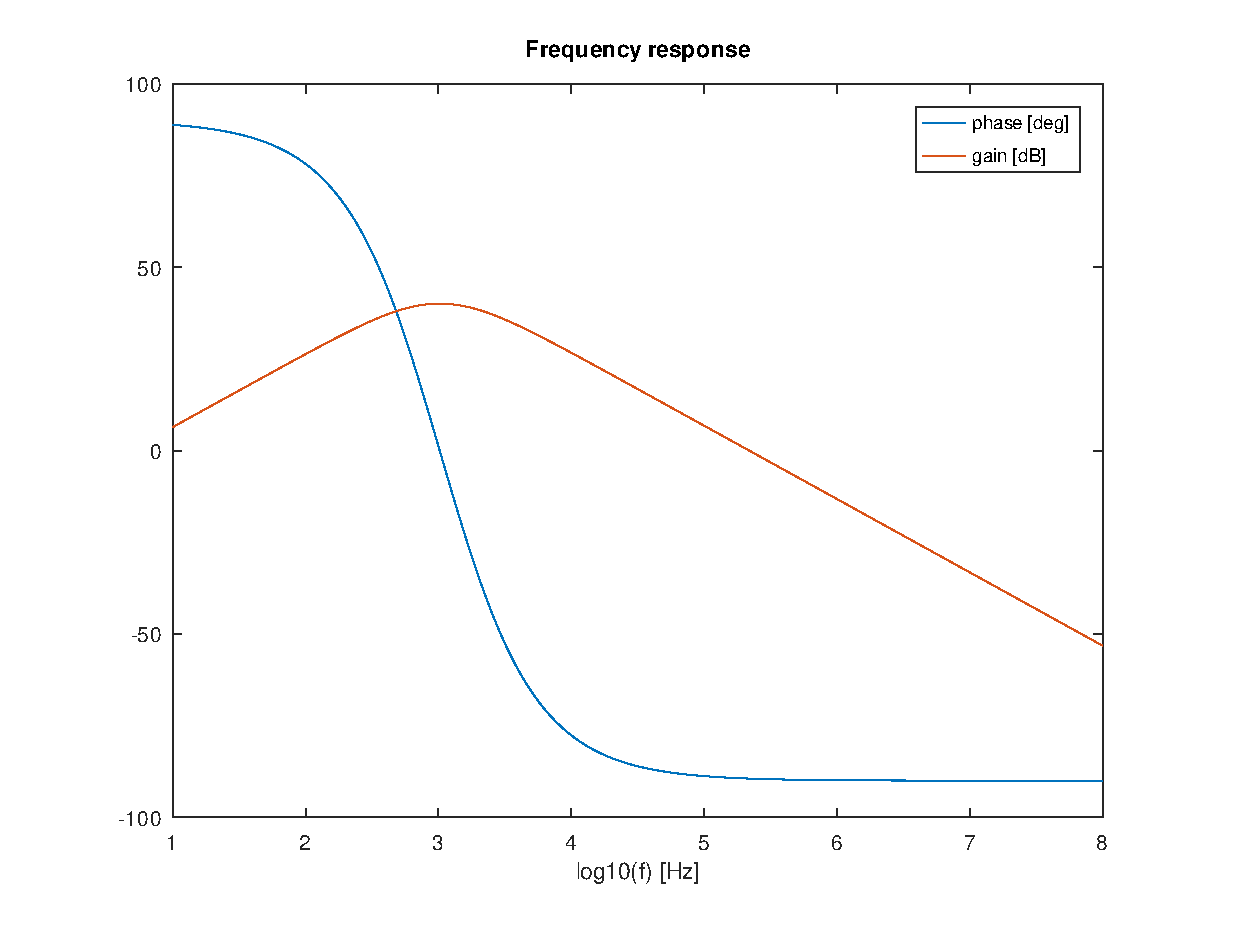
\includegraphics[width=0.4\linewidth]{theory.eps}
\caption{Frequency response for the simulation analysis}
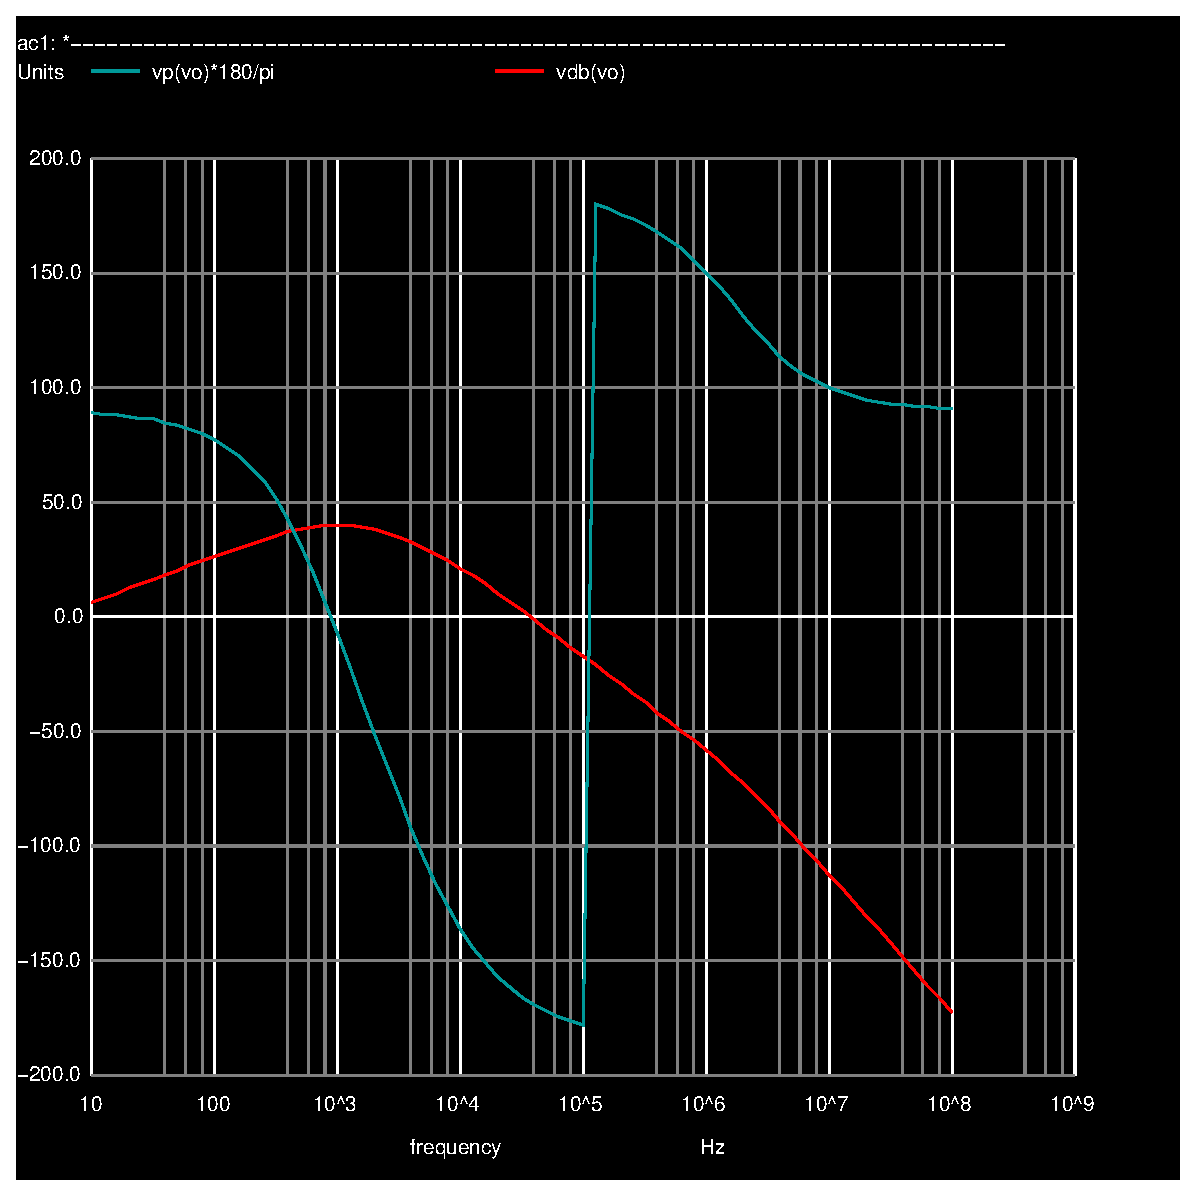
\includegraphics[width=0.4\linewidth]{simulation.eps}
\label{fig:theoretical}
\end{figure}
